\documentclass[11pt]{article}
\usepackage[english]{babel}
\usepackage[utf8]{inputenc}
\usepackage{fancyhdr}
\usepackage{amsmath}
\usepackage{amsfonts}
\usepackage{mathrsfs}
\usepackage{mathtools}
\usepackage{indentfirst}
\usepackage{hyperref}
\usepackage{tikz,amsmath}
\usepackage{tikz,tkz-tab,amsmath}
\usetikzlibrary{trees}
\usetikzlibrary{arrows}
\usepackage{cancel}
\usepackage{xfrac}  

\usepackage{minted}
\usepackage{lmodern}

\usepackage{enumerate}

%\setlength{\TPHorizModule}{1mm}
%\setlength{\TPVertModule}{1mm}
  
% to disable automat²ic indentation on new paragraphs
%\setlength{\parindent}{0pt}

\hypersetup{
    colorlinks=true,
    linkcolor=blue,
    filecolor=magenta,
    urlcolor=blue,
}
\urlstyle{same}

\parskip 1ex

\usepackage{pythonhighlight}

\usepackage{geometry}
 \geometry{
 a4paper,
 left=20mm,
 top=20mm,
 bottom=20mm,
 right=20mm
 }
\usepackage{multicol}
\pagestyle{fancy}
\fancyhf{}
\lhead{Matthieu Bessat}
\rhead{DM 12 - 27 janv. 2021}
\rfoot{Page \thepage}

\makeatletter
\def\@seccntformat#1{%
  \expandafter\ifx\csname c@#1\endcsname\c@section\else
  \csname the#1\endcsname\quad
  \fi}
\makeatother

\makeatletter
\renewcommand*\env@matrix[1][*\c@MaxMatrixCols c]{%
  \hskip -\arraycolsep
  \let\@ifnextchar\new@ifnextchar
  \array{#1}}
\makeatother

\newcommand{\vspacem}{\vspace{3mm}}
\newcommand{\bfrac}[2]{\displaystyle\frac{#1}{#2}}
\newcommand{\blim}[1]{\displaystyle\lim_{#1}}
\newcommand{\bbinom}[2]{\displaystyle\binom{#1}{#2}}
\newcommand{\N}{\mathbb{N}}
\newcommand{\R}{\mathbb{R}}

\newcommand\aug{\fboxsep=-\fboxrule\!\!\!\fbox{\strut}\!\!\!}
% just deleted a macro
%
%
%

\begin{document}
\enskip

\vspace{-10px}
\begin{center}
\fontsize{20pt}{20pt}\selectfont
\textbf{DM 12}
\end{center}
\fontsize{11pt}{11pt}\selectfont

\vspace{15px}

\setlength{\abovedisplayskip}{0pt}
\setlength{\belowdisplayskip}{0pt}
\setlength{\abovedisplayshortskip}{0pt}
\setlength{\belowdisplayshortskip}{0pt}

\textbf{1.}

\noindent On sait que $f$ est continue sur $I$ et que $f$ est strictement monotone sur $I$ car $f' > 0$ sur $I$. On sait aussi que f prends la valeur 0 en $\alpha \in I$. Alors d'après le théorème de la bijection : $\exists!\; \alpha \in I,\; f(\alpha) = 0$

\vspace{15px}
\noindent Ainsi :
\vspace{-15px}
\[\boxed{\alpha \text{ est l'unique réel vérifiant } f(\alpha) = 0}\]
\vspace{10px}

\textbf{2.a}

\noindent Soit $x_0 \in I$, l'équation de la tangente à la courbe de $f$ en  $x_0$ est : $\boxed{y = f(x_0) + f'(x_0)(x-x_0)}$

\vspace{10px}

\textbf{2.b.}

\noindent On cherche l'abscisse noté $x_{in}$ de l'intersection de la tangente en $x_0$ avec l'axe des abscisses.

\noindent On cherche $x_{in}$ tel que :
\vspace{5px}

\begin{align*}
f(x_0) + f'(x_0)(x_{in} - x_0) &= 0 &&\\
\Leftrightarrow f'(x_0)x_{in} - f'(x_0)x_0 &= -f(x_0) &&\\
\Leftrightarrow f'(x_0)x_{in} &= f'(x_0)x_0  - f(x_0) &&\\
\Leftrightarrow x_{in} &= \bfrac{f'(x_0)x_0}{f'(x_0)} - \bfrac{f(x_0)}{f'(x_0)} &&\\
\Leftrightarrow x_{in} &= x_0 - \bfrac{f(x_0)}{f'(x_0)} &&\\
\end{align*}

\vspace{5px}
\noindent Ainsi l'expression de l'abscisse est :
\vspace{-22px}
\[\boxed{x_{in} = x_0 - \bfrac{f(x_0)}{f'(x_0)}}\]


\vspace{15px}
\textbf{2.c}

\vspace{-25px}
\begin{center}
\includegraphics[scale=0.7]{output.png}
\end{center}

\noindent Avec $f: x \mapsto e^x - 2$ la suite $(u_n)_{n\in \N}$ semble converger vers $\alpha$ la racine de la fonction $f$.

\newpage
\textbf{3.a}

\noindent On étudie le signe de la différence.
\noindent On pose $\forall \; (t, x) \in \R^2, \quad \varphi(x) = f(x) - \big[f(t)+f'(t)(x-t)\big]$

$\varphi(x) = f(x) - \big[f(t)+f'(t)(x-t)\big]$

$\Leftrightarrow \varphi(x) = f(x)-f(t)-f'(t)(x-t)$

$\Leftrightarrow \varphi(x) = f(x)-f(t)-f'(t)x+f'(t)t$

\noindent On a $\varphi'(x) = f'(x)-f'(t)$ et  $\varphi''(x) = f''(x)$.

\noindent Or $f''\geq0$ donc $\varphi''\geq0$, ainsi $\varphi'$ est croissante. Vu que $\varphi'(t) = 0$ et $\varphi(t) = 0$, on a donc $\varphi \geq 0$. Comme illustré dans le tableau de variation suivant :

\vspace{8px}
\begin{center}
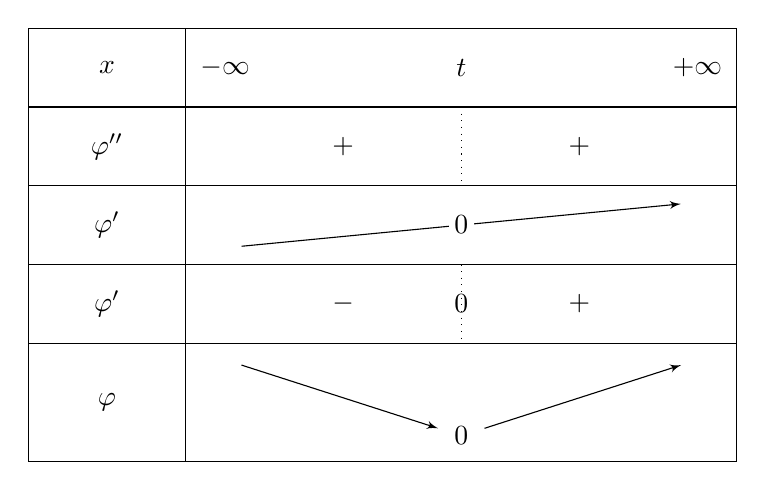
\begin{tikzpicture}
\tkzTabInit[]{$x$ /1, $\varphi''$ /1, $\varphi'$ /1, $\varphi'$ /1, $\varphi$ /1.5}{$-\infty$, $t$, $+\infty$}
\tkzTabLine{,+,t,+,}
\tkzTabVar{-/, R/, +/}
\tkzTabIma{1}{3}{2}{$0$}
\tkzTabLine{,-,z,+,}
\tkzTabVar{+/, -/$0$, +/}
\end{tikzpicture}
\end{center}
\vspace{12px}
\noindent Ainsi :
\vspace{-12px}
\[\boxed{\forall\; (x, t) \in \R^2, \;\; f(x) \geq f(t) + f'(t)(x-t)}\]

\vspace{12px}
\textbf{3.b}

\noindent On utilise l'inégalité de la question précédente en posant $t = u_n$ et $x= \alpha$ :
\begin{align*}
f(\alpha) &\geq f(u_n) + f'(u_n)(\alpha-u_n) &&\\
\Leftrightarrow f(\alpha) &\geq f(u_n)+f'(u_n)\alpha - f'(u_n)u_n &&\\
\Leftrightarrow 0 &\geq f(u_n) + f'(u_n)\alpha - f'(u_n)u_n &&\\
\Leftrightarrow f'(u_n)u_n - f(u_n) &\geq f'(u_n)\alpha &&\\
(\text{car } f' > 0 ) \Leftrightarrow u_n - \bfrac{f(u_n)}{f'(u_n)} &\geq \alpha &&\\
\Leftrightarrow u_{n+1} &\geq \alpha
\end{align*}

\vspace{12px}
\noindent Donc :
\vspace{-13px}
\[\boxed{\forall\; n \in \N, \;\; u_{n+1} \geq \alpha}\]

\vspace{5px}

\noindent Pour montrer que $(u_n)_{n\in\N^*}$ est décroissante on étudie le signe de $u_{n+1} - u_n$.

$u_{n+1}-u_n = u_n - \bfrac{f(u_n)}{f'(u_n)} - u_n = -\bfrac{f(u_n)}{f'(u_n)}$

\noindent On a $f' > 0$.

\noindent On a aussi pour tout entier $n > 0$, $u_n \geq \alpha \Leftrightarrow f(u_n) \geq f(\alpha) \Leftrightarrow f(u_n) \geq 0$ (Car $f$ est croissante)

Ainsi $\forall \; n \in \N^*, \;\; \bfrac{f(u_n)}{f'(u_n)} \geq 0$ c'est-à-dire $u_{n+1}-u_n \leq 0$

\vspace{12px}
\noindent On en conclut :
\vspace{-15px}
\[\boxed{(u_n)_{n\in\N^*} \text{ est décroissante}}\]

\newpage
\textbf{3.c}

\noindent Vu que $(u_n)_{n\in\N^*}$ est minoré par $\alpha$ et décroissante, cette suite admet une limite noté $l$ finie et supérieure à $\alpha$.

\noindent Ainsi $(u_n)$ et $(u_{n+1})$ (suite extraite) admettent la même limite $l$. Ce qui donne que $u_{n+1} - u_n \longrightarrow 0$. 

\noindent Également on a (par passage à la limite) : $-\bfrac{f(l)}{f'(l)} \longrightarrow 0$

\noindent Or on sait que $f' > 0$, on déduit que $f(l) = 0$, d'après la question 1, il y a unicité de la racine de $f$ donc $l = \alpha$

\vspace{8px}
\noindent Ainsi $(u_n)_{n\in\N^*}$ converge et :
\vspace{-15px}
\[\boxed{u_n \longrightarrow \alpha}\]

\vspace{10px}
\textbf{4.a}
\begin{python}
def derive(f, a):
    h = 1e-10
    return (f(a+h)-f(a))/h
\end{python}


\vspace{10px}
\textbf{4.b}
\begin{python}
def newton(f, u0, n):
    u = u0
    for i in range(n):
        u = u-f(u)/derive(f, u)
    return u
\end{python}


\vspace{10px}
\textbf{4.c.i}

$g: x \mapsto e^x-2$

$g': x \mapsto e^x$ donc $g' > 0$ et est continue

$g'': x \mapsto e^x$ donc $g'' \geq 0$ et est continue

\noindent Ainsi $g$ est de classe $\mathcal{C}^2$.

\noindent Vu que $g$ est continue et strictement monotone et prends des valeurs dans $\R$ sur $\R$ alors d'après le théorème de la bijection, il existe un unique réel $\beta$ tel que $g(\beta) = 0$.

\noindent Cherchons $\beta$ : $e^{\beta} - 2 = 0 \Leftrightarrow e^{\beta} = 2 \Leftrightarrow \beta = \ln(2) \approx 0.69$

\noindent En conclusion :
\vspace{8px}
\[\boxed{\text{La fonction } g \text{ vérifie bien les hypothèses de la méthode de Newton et la racine est} \ln(2).}\]

\vspace{15px}
\textbf{4.c.ii}

\vspace{-5px}
\renewcommand{\arraystretch}{1.5}
\begin{center}
\begin{tabular}{ c|c|c }
 $n$ & $u_n$ & $|u_n - \ln(2)|$ \\ 
 \hline
 \hline
 2 & 0.6940423612292895 & 0.0008951806693442421 \\
 \hline
 3 & 0.6931475805255273 & 3.9996558198751586e-07 \\ 
 \hline
 4 & 0.6931471805598984 & 4.6851411639181606e-14 \\ 
 \hline
 5 & 0.6931471805599453 & 0.0 \\ 
 \hline
\end{tabular}
\end{center}

\newpage
\textbf{5.a}

\noindent Soit $r\in\R^*_+$, on étudie la fonction $h: x \mapsto x^2-r$ sur $\R$. On a donc :

$h': x \mapsto 2x$ donc $h' > 0$ et $h$ est continue sur $\R$.
$h'': x \mapsto 2$ donc $h'' \geq 0$ et $h''$ est continue sur $\R$

\noindent Ainsi $h$ est de classe $\mathcal{C}^2$.

\noindent L'intervalle $\R^*_+$ est la seule intervalle possible qui respecte les hypothèses (2) et (3) de la méthode de Newton.

\noindent De plus, vu que $h$ est continue et strictement monotone sur $R^*_+$, le théorème des valeurs intermédiaire donne : $\exists \; \alpha \in \R^*_+, \;\; h(\alpha) = 0$

\begin{center}
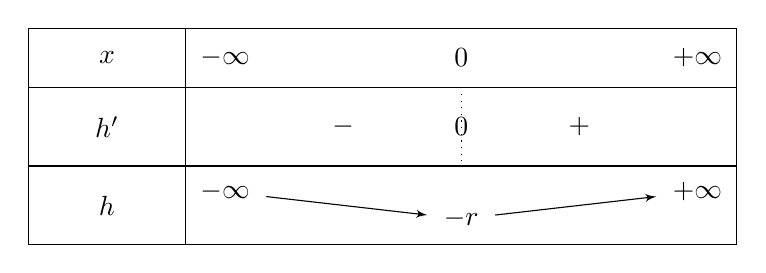
\begin{tikzpicture}
\tkzTabInit[]{$x$ /.75, $h'$ /1, $h$ /1}{$-\infty$, 0, $+\infty$}%
\tkzTabLine{,-,z,+,}
\tkzTabVar{+/$-\infty$, -/$-r$, +/$+\infty$}
\end{tikzpicture}
\end{center}

\noindent En conclusion :
\boxed{\text{La fonction } h \text{ vérifie bien les hypothèses de la méthode de Newton.}}

\vspace{15px}
\textbf{5.b}

\noindent En utilisant la suite définit à la question 2.c on a :

$u_{n+1} = u_n - \bfrac{h(u_n)}{h'(u_n)} = u_n - \bfrac{u_n^2 - r}{2u_n}$

$u_{n+1} = \bfrac{2u_n^2 - u_n^2 + r}{2u_n}  = \bfrac{u_n^2 + r}{2u_n}$

\vspace{5px}

\noindent Ainsi la relation de récurrence de la suite associée à la méthode de Newton est :

\vspace{5px}
\[\boxed{u_{n+1} = \bfrac{u_n^2 + r}{2u_n}}\]

\vspace{12px}
\textbf{5.c}
\begin{python}
def rc(r, n):
  u = 1
  for i in range(n):
    u = (u**2+r)/(2*u)
  return u
\end{python}

\vspace{10px}
\textbf{5.d}
\begin{python}
def rc2(r,p):
  u0, u1 = 1, p+2
  while abs(u0 - u1) >= p:
    u0 = u1
    u1 = (u0**2+r)/(2*u0)
  return u1
\end{python}

\end{document}

